\chapter{Implementace}
V této kapitole bude obsažen popis implementace návrhu z předchozích kapitol. Budou zde do detailu rozebrány jednotlivé části implementace a popsány problémy, které se vyskytly během vývoje. Dále bude popsána spolupráce na vývoji a nástroje, které byly použity k usnadnění této spolupráce.

\section{Komunikace s API}
Komunikace s API byla implementována pomocí XMLHttpRequest, který je součástí JavaScriptu. Byly vytvořeny čtyři základní funkce, které slouží k odesílání dotazů na API. Tyto funkce jsou \texttt{get}, \texttt{post}, \texttt{put} a \texttt{delete}. Každá z nich má čtyři parametry: URL dotazu, token, úspěšný callback a neúspěšný callback. Token je autorizační token, který je nutné přidat do hlavičky většiny dotazů, aby bylo možné je provést. Token není vždy povinný, ale většina dotazů ho vyžaduje. Úspěšný callback je funkce, která se provede v případě úspěšného dotazu a neúspěšný callback je funkce, která se provede v případě, kdy API vrátí chybu. Funkce \texttt{post} a \texttt{put} navíc mají ještě pátý parametr, kterým jsou data. Tato data jsou v dotazu předána API a jsou dále zpracována podle toho, o jaký dotaz se jedná. Ukázku implementace jedné z těchto funkcí lze najít v ukázce \ref{code:post_request} a její užití v jednom z jednodužších případů v ukázce \ref{code:post_usage}.

\begin{listing}[H]
  \inputminted[breaklines]{typescript}{resources/code/post_request.ts}
  \caption{Implementace funkce pro odeslání POST dotazu}
  \label{code:post_request}
\end{listing}

\begin{listing}[H]
  \inputminted[breaklines]{typescript}{resources/code/post_usage.ts}
  \caption{Použití funkce pro odeslání POST dotazu}
  \label{code:post_usage}
\end{listing}


\section{Databáze}
Databáze byla vyvíjena za účasti všech řešitelů tohoto projektu. Je implementována v MariaDB, což je open-source odvětví MySQL databáze. Ta nám byla díky její spolehlivosti doporučena vedoucím práce. Databáze se v průběhu vývoje měnila, jelikož se měnila i struktura dat, které byly potřeba ukládat. V současné době obsahuje 48 tabulek, z čehož 11 z nich slouží čistě jako vazební. Databáze je přístupna pouze z backendové části aplikace, přes koncové body API. Schéma celé databáze (bez vazebních tabulek) je zobrazeno na obrázku \ref{fig:db_schema}.

\begin{figure}[htbp]
  \centering
  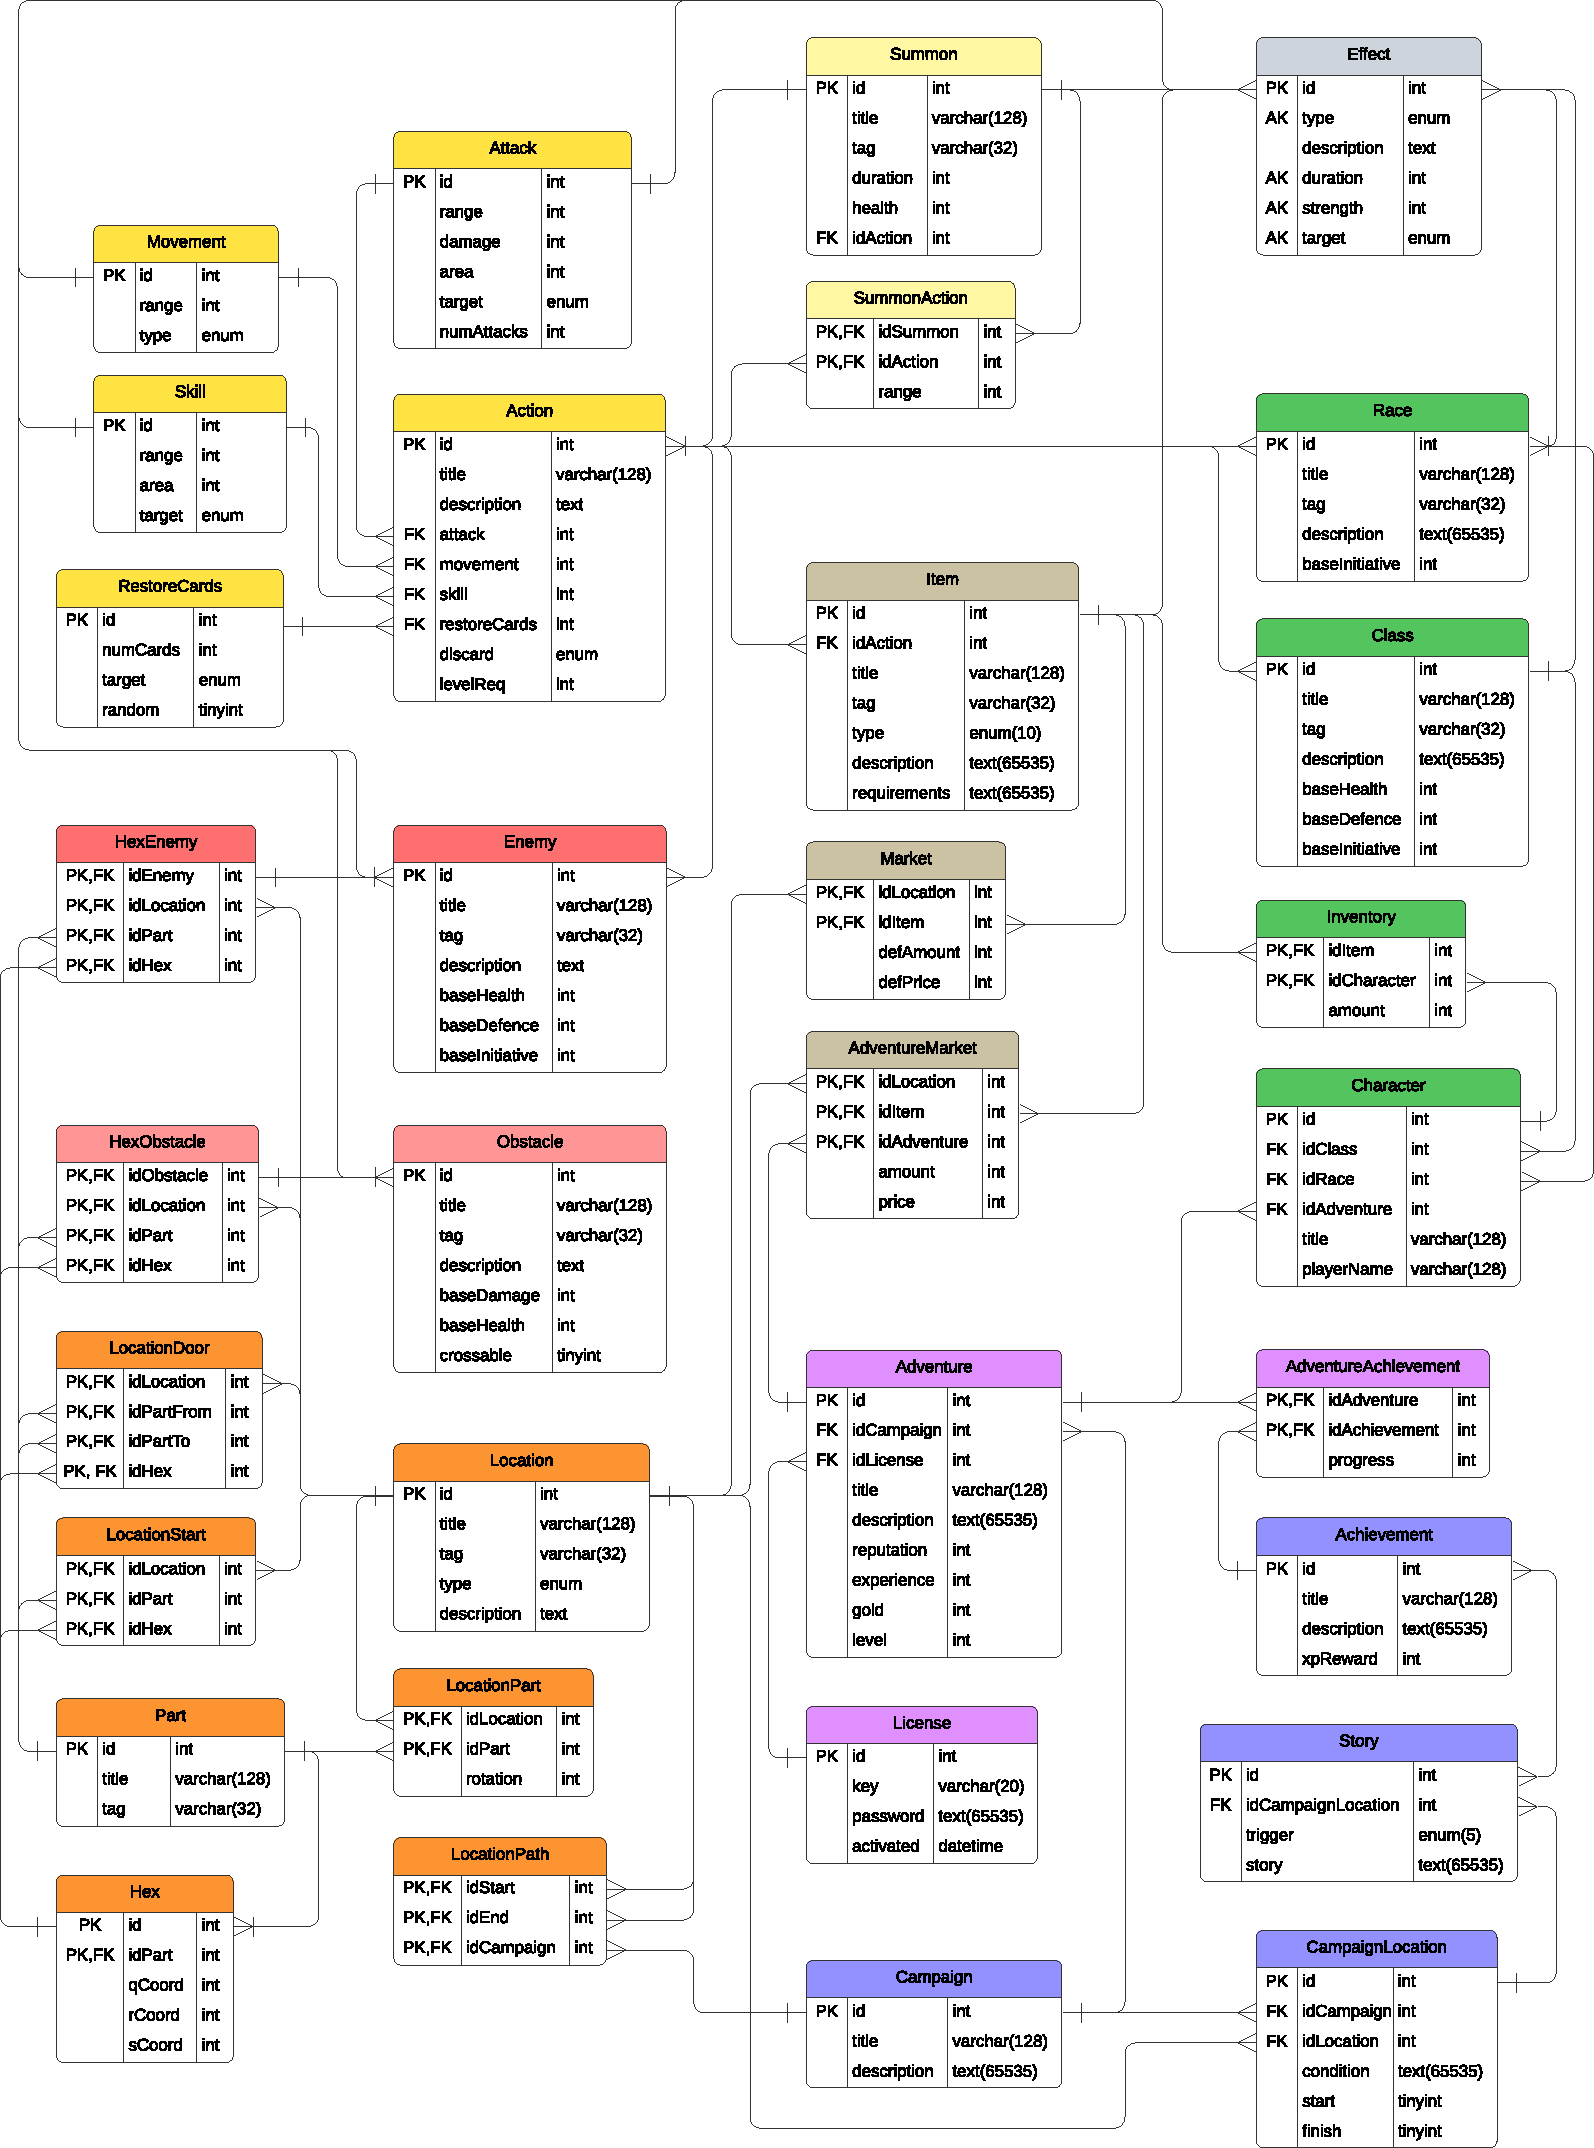
\includegraphics[width=.95\textwidth]{../../shared/diagrams/dbScheme.pdf}
  \caption{Schéma databáze}
  \label{fig:db_schema}
\end{figure}

\section{Stránky frontendové aplikace}
V následující sekci budou popsány jednotlivé stránky, které byly implementovány v rámci frontendové části této práce. Všechny komponenty, které jsou součástí těchto stránek, byly implementovány tak, aby byly co nejvíce modulární a znovupoužitelné. Bylo také dbáno na to, aby byly co nejvíce odděleny od zbytku aplikace, což by mělo zjednodušit případné budoucí úpravy a rozšíření. Komponenty komunikují s backendem pomocí API, které bylo implementováno kolegy, se kterými jsem se spolupodílel na tomto projektu.

\subsection{Přihlašování}
Přihlašování je první komponenta, která je uživateli po navštívení stránky zobrazena. Jedná se o jednoduchý formulář se dvěma poli, kde uživatel zadá své licenční číslo a heslo. Po potvrzení formuláře se data odešlou na server, kde se porovnají s daty v databázi. Pokud je vše v pořádku, tak se z API vrátí odpověď s tokenem a identifikátorem licence a obě tyto informace se uloží do relace. Token se dále používá pro autorizaci dotazů. Následně je uživatel přesměrován na další komponentu. V případě, že je příhlášení chybné, je uživateli zobrazena chybová hláška pomocí knihovny Notiflix. Jedná se o jednoduchou komponentu, která nevyžaduje žádné složité operace, tudíž ani její implementace nebyla nijak náročná.

\subsection{Výběr dobrodružství}
Tato komponenta následuje hned po přihlášení. Zde si může uživatel prohlédnout, vybrat, či vytvořit takzvané dobrodružství (ta jsou stručně popsáne zde: \ref{sec:adventure}). Každé z nich má vlastní kartu, která obsahuje název, popis a výčet zdrojů, které mají hráči dostupné. Uživatel si může vybrat dobrodružství, které chce hrát, a následně je přesměrován na další komponentu. Pokud si žádné nevybere, může si vytvořit nové. Vytvoření nového dobrodružství je možné pouze v případě, že jich na dané licenci existuje méně než osm, což by mělo být dostatečné množství. Zároveň je zde možnost dobrodružství smazat, či upravit jeho název a popis.

U této komponenty se projevil problém s rozlišováním jednotlivých karet s dobrodružstvími. Svelte framework umožnujě použití cyklů, které byly využity pro vytvoření karet. Problém nastal při pokusu o přidání funkcí pro smazání a úpravu. Tyto funkce byly implementovány pomocí modálních oken, které se zobrazí po kliknutí na tlačítko na kartě. Problém byl v tom, že všechny karty měly stejný identifikátor, tudíž nebylo možné rozlišit, která z nich byla vybrána. Tento problém byl vyřešen přesunutím karty a modálního okna do samostatné komponenty, která si udržuje svůj vlastní stav. Podobný problém s identifikátory se v tomto projektu vyskytl několikrát a vždy byl vyřešen obdobným způsobem.

Další problém se naskytl, když jsem se pokusil dynamicky měnit barvu svg obrázku, který je použit na tlačítku pro přidání nového dobrodružství. Při pokusu o změnu barvy pomocí standardních CSS vlastností nenastala žádná změna. Tento problém byl vyřešen přidáním vlastnosti \texttt{filter}, která umožňuje aplikovat obrázkům různé efekty pomocí několika barevných filtrů. Tyto filtry zahrnují mimo jiné také \texttt{brightness}, \texttt{contrast}, \texttt{sepia}, \texttt{saturate}, \texttt{hue-rotate} a \texttt{invert}, které byly pro potřebnou změnu barvy použity. Z původní černé byly takto vytvořeny barvy světle šedá (s hexadecimální hodnotou \texttt{\#bababa}) pro výchozí stav a tmavě šedá (\texttt{\#222}) pro stav po najetí myši. Tyto světlé barvy odpovídají těm použitým ve zbytku aplikace. Ukázka kódu, kterým byla tato změna provedena, je uvedena v ukázce \ref{code:svg_filter}. Tento problém nebylo složité vyřešit, ale jeho řešení jsem považoval za zajímavé, jelikož je nutné barvu aproximovat pomocí filtrů, místo aby bylo možné ji nastavit přímo.

\begin{listing}[H]
  \inputminted[breaklines]{css}{resources/code/svg_color.css}
  \caption{Změna barvy svg obrázku pomocí CSS filtrů}
  \label{code:svg_filter}
\end{listing}

\subsection{Vytvoření postav}
Pokud si uživatel vytvoří nové dobrodružtví, či si vybere nějaké, ve kterém prozatím nejsou žádné postavy, je přesměrován na tuto komponentu. Zde si může vytvořit až šest postav, které budou v daném dobrodružtví učinkovat. Každé z postav hráč přiřadí jméno, jméno hráče a dále vybere její rasu a povolání. Ty společně určují hráčovy statistiky, jako body životů, obranu a iniciativu. Každá rasa a povolání má svůj vlastní obrázek, který ji představuje. Pod každým z nich se také nachází tlačítko, které zobrazí popis dané rasy, či povolání v podobě okénka nápovědy. Po vybrání obou možností se také zobrazí finální obrázek postavy, který odpovídá kombinaci zvolených možností. Zároveň se při změně jedné z nich změní jak obrázek, tak i výpis statistik. Ukázku této komponenty lze najít na obrázku \ref{fig:character-creation}.

U této komponenty bylo nejvíce práce s grafickým zpracováním. Bylo potřeba vytvořit kvalitně vyhlížející obrázky pro všechny rasy a povolání, což bylo poměrně časově náročné. Dále bylo potřeba vytvořit algoritmus, který na základě zvolených možností vybere správný obrázek. Tento algoritmus byl implementován pomocí jednoduchého pravidla, kde se odkaz na obrázek skládá z názvu rasy a povolání.

Použitá okna nápovědy byla importována z knihovny Bootstrap. Vyvstal u nich menší problém, kdy se kvůli způsobu jejich inicializace přestaly zobrazovat po změně obsahu. Tento problém byl vyřešen přidáním vlastního kódu, který okénka znovu inicializuje po každé změně.

\begin{figure}[H]
  \centering
  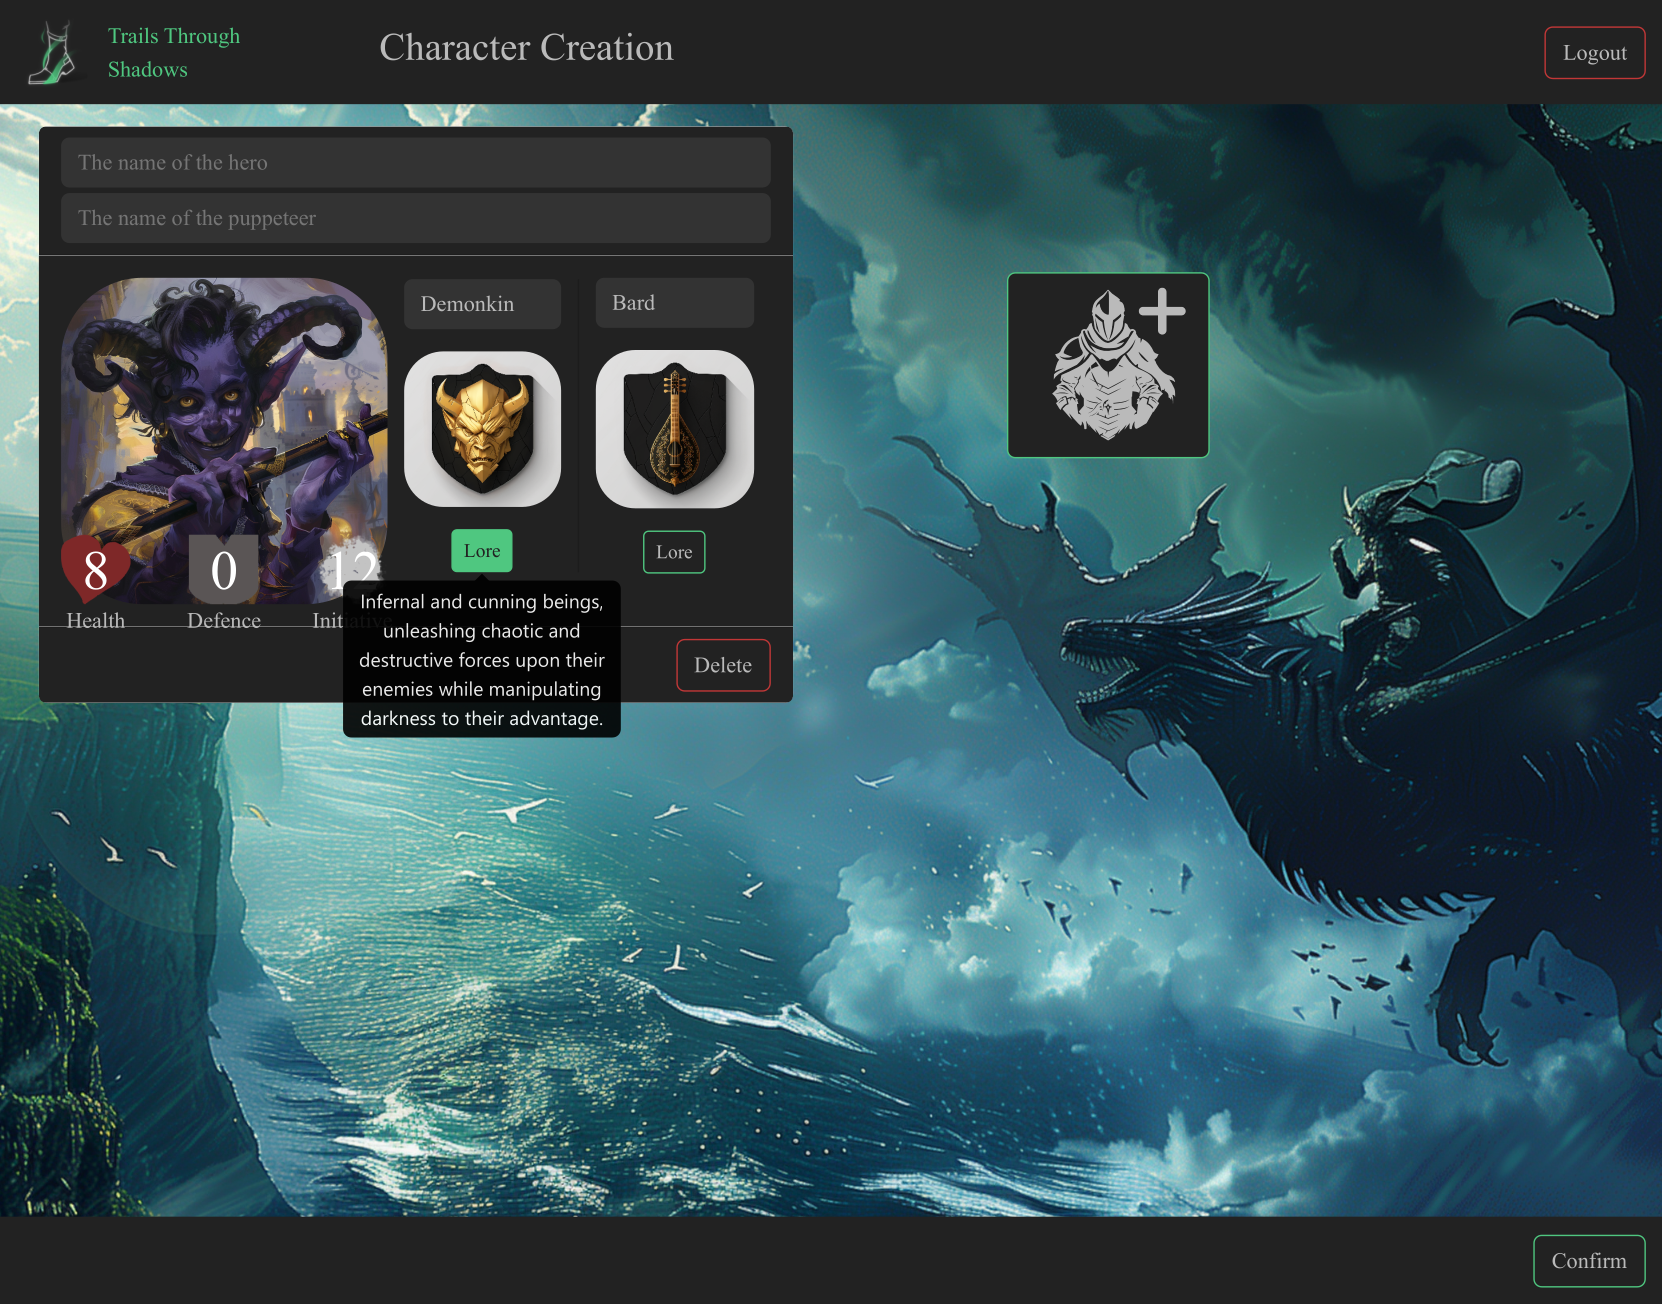
\includegraphics[width=.95\textwidth]{resources/figures/TTS-Charracter Creation.pdf}
  \caption{Snímek obrazovky komponenty pro vytváření postav}
  \label{fig:character-creation}
\end{figure}

\subsection{Dobrodružství a přehled postav}
Po vytvoření postav je uživatel přesměrován na tuto komponentu, kde si může prohlédnout všechny postavy, které v daném dobrodružství vytvořil. Každá z nich má svou kartu, která obsahuje jméno, jméno hráče, rasu, povolání, statistiky a její předměty. Zároveň se zde nechází tlačítko, které uživateli dovolí začít nové střetnutí, či pokračovat v dříve započlém.

\subsection{Střetnutí}
Tato komponenta je nejkomplexnější a také nejdůležitější ze všech. Jedná se již totiž o samotnou hru. Uživateli je jako první věc zobrazen příběh daného střetnutí, který slouží jako clona, jež maskuje načítání a vykreslování dat. Střetnutí může mít několik různých ukončovacích podmínek, které jsou zde také vypsány. Kvůli komplexity této komponenty bude popsána podrobněji v následujících sekcích.

\subsubsection*{Mapa}
Po odkliknutí příběhu je zobrazena hrací plocha ukazující první místnost s tokeny nepřátel a překážek, dveřmi a startovacími poli pro postavy. Ta slouží jako návrh pro fyzickou hrací plochu, kterou hráč podle této předlohy připraví. Tokeny nepřátel a pastí jsou zmenšené, detailnější obrázky jejich protějšků, kterým byl pro lepší pŕehlednost přidán barevný okraj. Mapa také vyobrazuje dveře, které vedou do dalších místností. Při kliknutí na ně se uživateli zobrazí možnost je otevřít. Vyhodnocení otevření dveří se provede vždy na konci kola. Potom co se tak stane se krom stávající místnosti zobrazí také nová a uživatel může přepínat mezi jednotlivými náhledy pomocí tlačítek na okraji mapy. Ukázku této komponenty lze najít na obrázku \ref{fig:map}.

\begin{figure}[H]
  \centering
  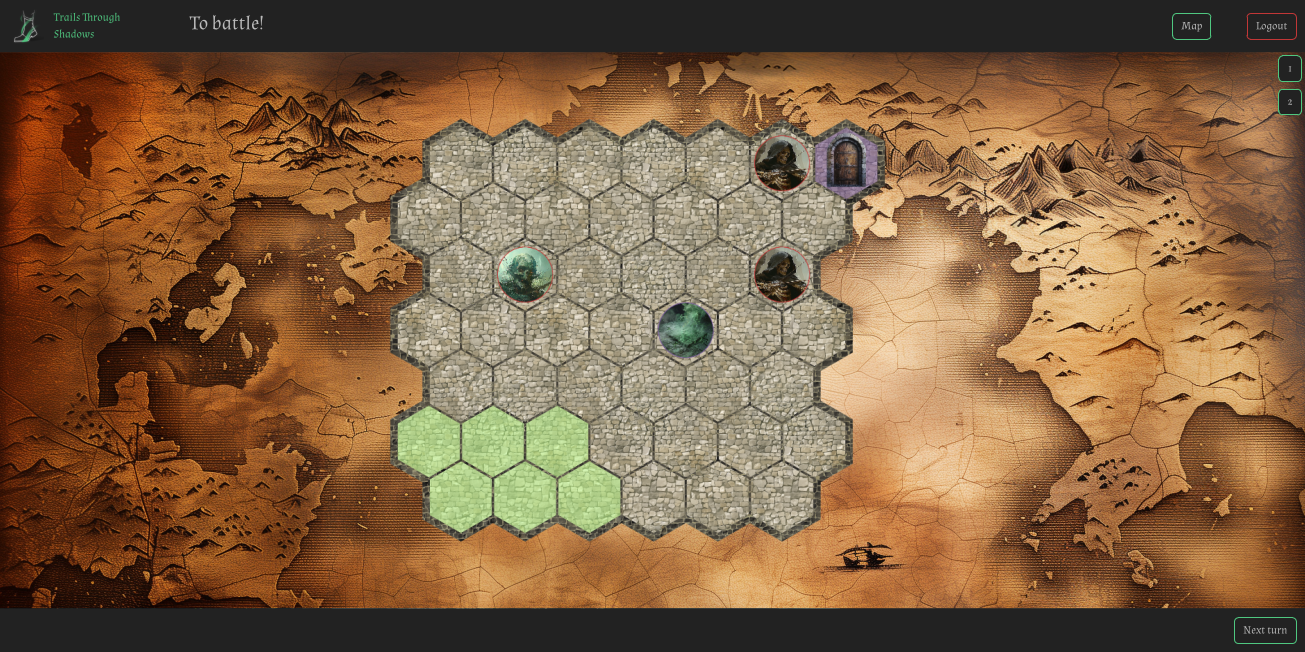
\includegraphics[width=.95\textwidth]{resources/figures/TTS-Map.pdf}
  \caption{Snímek obrazovky komponenty pro mapu}
  \label{fig:map}
\end{figure}

Mapa je vykreslena pomocí HTML elementu kanvas, který umožňuje vykreslování grafiky pomocí JavaScriptu. Pro tento účel bylo navrženo několik funkcí, které umožňují vykreslit jednotlivé části mapy, jako jsou místnosti, tokeny a dveře. Tyto funkce jsou volány vždy při změně stavu, která se týká mapy a to včetně změny velikosti okna. Tímto způsobem je zajištěno, že se mapa vždy zobrazuje správně a všechny změny jsou ihned viditelné. Při změně místnosti se například vykreslí nová místnost a všechny tokeny, které se v ní nachází. Při otevření dveří se zase zobrazí nová místnost a všechny tokeny, které se v ní nachází. 

Jelikož se jedná o pole hexagonálního tvaru, bylo pro účel vykreslování rozhodnuto o používání kubického souřadného systému, který počítá se třemi souřadnicemi. Tento systém je výhodný pro práci s hexagony, jelikož umožňuje snadno vypočítat jejich pozici a sousedy. Na tuto soustavu bylo nutné si nějakou dobu zvykat a vytvořit si vlastní funkce pro práci s ní. Výsledný kód je ale díky tomu mnohem čitelnější a jednodušší na úpravy.

Dále je pro lepší viditelnost implementována funkce, která zajišťuje zvýraznění pole, nad kterým se nachází kurzor myši. Ta je volána při každém pohybu myši a zajišťuje uživateli lepší orientaci na mapě a odezvu na jeho akce.

\subsubsection*{Iniciativa}
Dále jsou zobrazeny postavy, včetně obrázku a jména a jsou uspořádány do jednotlivých karet. Před započetím samotného střetnutí je hráč vyzván k zadání iniciativy pro každou z postav. Iniciativa je číslo, které určuje pořadí, ve kterém postavy a nepřátelé jednají. Entita na tahu je zvýrazněna pomocí zvětšení celé její karty.

Výběr iniciativy je implementován pomocí jednoduchého výběru z rozbalovacího seznamu. Výběr zahrnuje všechny hodnoty, které si hráč může hodit na kostce (ty lze najít zde \ref{tab:dice_symbols}). Iniciative nepřátel je získána pomocí API.

\subsubsection*{Střetnutí}
Po zadání iniciativy je zobrazena hlavní část střetnutí, kde se karty s postavami a nepřáteli seřadí podle hodnoty iniciativy. Zde se entity střídají se svými tahy v pořadí určeném iniciativou. Nepřátelé jsou rozděleni do skupin podle jejich typu. Pokud je na řadě nepřítel, API vrátí jeho akci, která je zobrazena uživateli. Pokud je na řadě postava, uživatel si své akce vybírá z fyzických karet, které má k dispozici. Všechny akce vyhodnocuje sám uživatel, který má k dispozici interface, který umožňuje entitám ubírat životy a přidávat efekty. Pokud jsou otevřeny dveře, okamžitě po vyhodnocení se ke stávajícím nepřátelům přidají noví a zařadí se do iniciativy. Střetnutí končí v okamžik, kdy je splněna jedna z podmínek pro výhru, či prohru. V ten moment je uživatel přesměrován na finální obrazovku, kde je zobrazen výsledek střetnutí a následně zpět na přehled postav. Ukázku této komponenty lze najít na obrázku \ref{fig:combat}.

\begin{figure}[H]
  \centering
  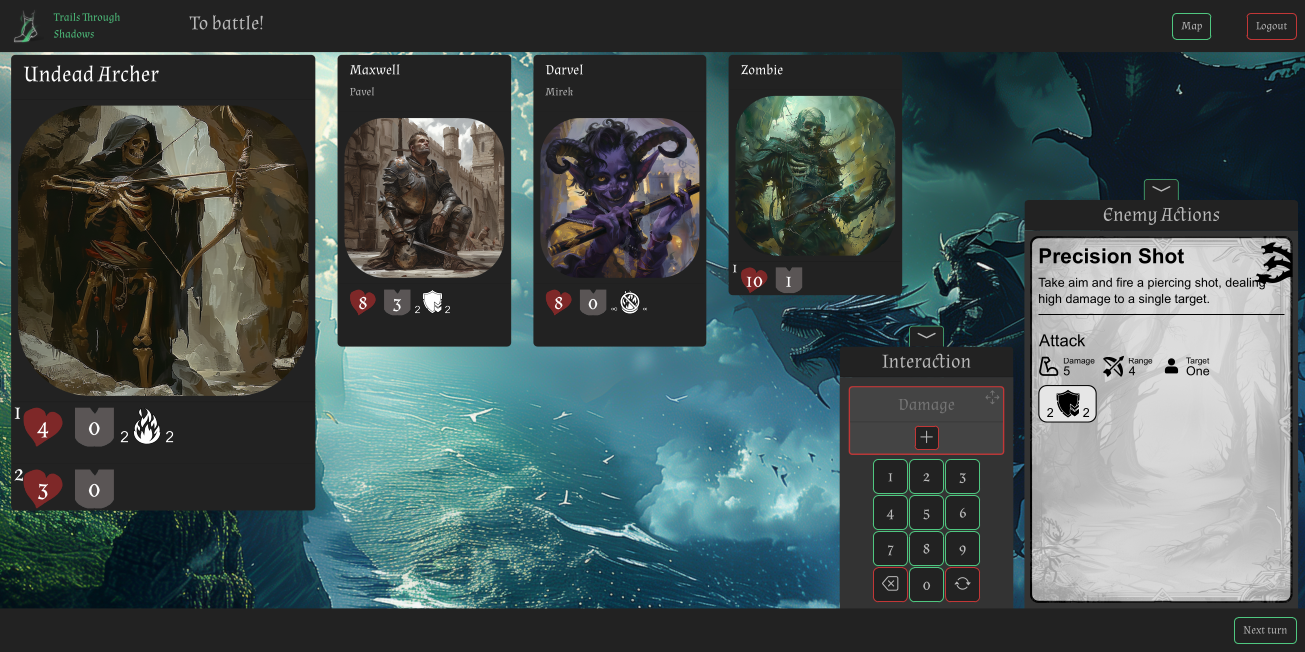
\includegraphics[width=.95\textwidth]{resources/figures/TTS-Encounter.pdf}
  \caption{Snímek obrazovky komponenty pro střetnutí}
  \label{fig:combat}
\end{figure}

Tato komponenta byla nejsložitější a nejvíce časově náročná ze všech. Bylo zde potřeba implementovat mnoho funkcí, které zajišťují správné chování střetnutí a jeho častou komunikaci s API. Nejvíce problémů nastalo při konci respektive začátku tahu jednotlivých entit. Bylo nutné kontrolovat, zda entita, která je na řadě, během svého tahu nezemřela. Pokud ano, bylo nutné ji ze seznamu odebrat, ukončit její tah a začít tah entity následující. Podobný problém se objevil také při implementaci efektů, kdy některé z nich způsobují zranění na začátku kola. Tím se mohlo stát, že entita sice započala svůj tah, ale zemřela hned poté bez možnosti cokoliv udělat a hra nebyla schopna ukončit její tah. Tento problém byl vyřešen přidáním kontrolní hodnoty v odpovědi z API na začátku každého tahu, zda je entita stále naživu. Pokud ne, tak se její tah přeskočí a začne tah entity následující.

Problémy také nastaly při spojování nepřátel do skupin. Bylo nutné zajistit, aby měl uživatel stále přehled o všech nepřátelích a jejich stavech. Tento problém byl původně vyřešen možností přepínáním mezi jednotlivými nepřáteli ve skupině, avšak toto se ukázalo jako velmi neohrabané a nepřehledné. Proto bylo rozhodnuto, že se na úkor jednolitosti karet zobrazí statistiky všech nepřátel ve skupině pod sebou.

Další problém se objevil při implementaci karet s akcemi, které byly původně implementovány jako HTML elementy. Tyto karty byly ale příliš komplikované pro výpis všech atributů a těžko se s nimi pracovalo. Proto bylo rozhodnuto je nahradit generovanými svg obrázky. Tímto způsobem bylo dosaženo lepšího vzhledu a snadnější práce s nimi.

\subsubsection*{Interface pro interakci s entitami}
Pro interakci s entitami byla vytvořena jednoduchá komponenta, která dává hráči možnost vepsat, či pomocí tlačítek zvolit, kolik životů má entita ztratit a pomocí modálního okna zvolit, který efekt má být na entitu aplikován. Tato komponenta je použita vždy, když je potřeba vyhodnotit útočnou akci, a to včetně akcí nepřátel a poškození způsobené překážkami.

Jedná se o komponentu která byla navržena primárně pro použití myší, k čemuž přispívá jak její grafické zpracování, tak i způsob ovládání. Hlavním ovládacím prvkem je virtuální klávesnice, která lze aktivovat právě myší. Způsob, kterým se vybírá cíl útoku, je založen na přetáhnutí ukazatele poškození na vybranou entitu. Tento způsob ovládání byl zvolen, jelikož je intuitivní, snadno pochopitelný a navíc podporuje možnost znovupoužití hodnot útoku pro více nepřátel.

\section{Spolupráce na vývoji}
Spolupráce probíhala převážně pomocí verzovacího systému Git a platformy GitHub, kde byl vytvořen repozitář pro Trails Through Shadows. V průběhu vývoje bylo vytvořeno několik větví, které sloužily k implementaci nových funkcí, opravám chyb a testování nových návrhů. Většina z nich byla následně sloučena zpět do hlavní větve, kde byly testovány a připravovány pro nasazení. Rozdělení práce je zobrazeno v blokovém shcématu \ref{fig:workflow}.

\begin{figure}[H]
  \centering
  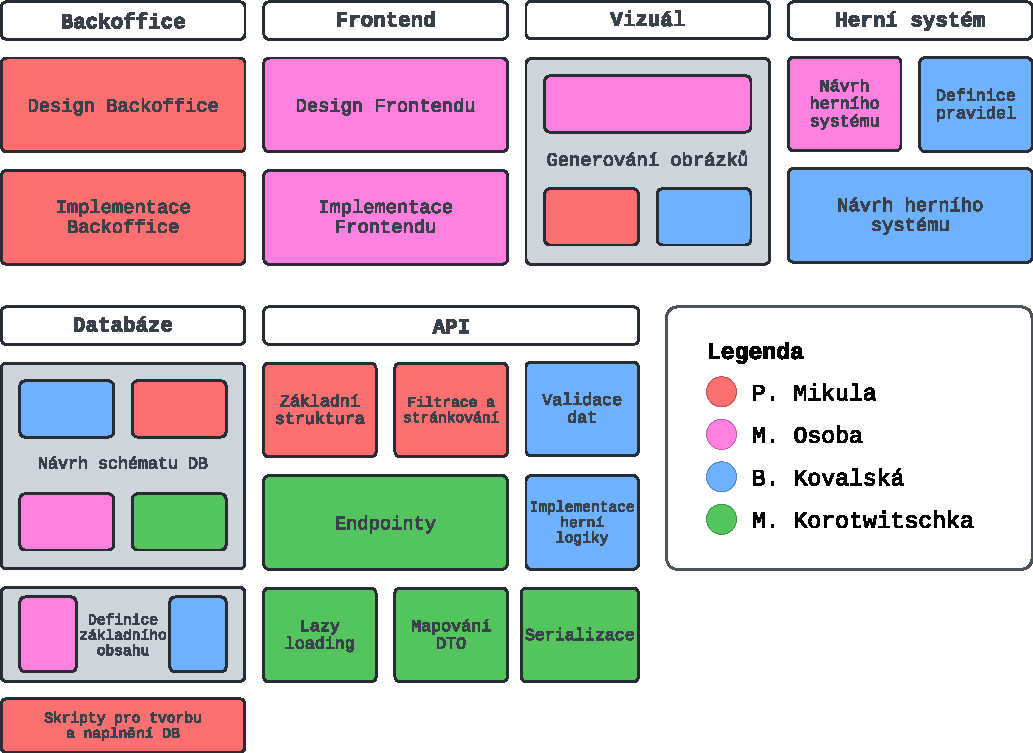
\includegraphics[width=.95\textwidth]{../../shared/diagrams/blocks.pdf}
  \caption{Blokové schéma rozdělení práce}
  \label{fig:workflow}
\end{figure}

Některé specifické části práce byly řešeny za pomoci specializovaných nástrojů. Databáze byla společně navržena pomocí programu dbdiagram.io, který dovoluje úpravu schématu databáze v reálném čase několika uživatelům najednou. Poznámky a prvotní návrhy pravidel a obecné funkčnosti byly zaznamenávány pomocí Google Docs. Většina komunikace pak probíhala přes platformu Discord, kde byly řešeny problémy, plánovány úkoly a konzultovány návrhy. Tato platforma byla také použita ke generování obrázků pomocí Midjourney a v neposlední řadě nám umožnila testování za pomoci několika velmi důsledných testerů.

Spolupráce nebyla vždy bezchybná a občasně se problémy vyskytly. Největším problémem byla komunikace mezi frontendovou a backendovou částí aplikace. V některých případech bylo obtížné dohodnout se na formátu a obsahu dat, které se mezi nimi přenášely. V jiných případech se muselo čekat, až jeden z týmů dokončí svou část, než mohla být otestována a následně zahájen vývoj druhé části. Tento problém se však postupem času stával méně častým, když se týmy naučily lépe spolupracovat a komunikovat.